% 5.4.      Magnetismo terrestre, brújula, giróscopo direccional libre.
% version 2019

\section{Magnetismo terrestre, br\'ujula, gir\'oscopo direccional libre}
\label{sec:magnetismo.terrestre}


\subsection{Magnetismo terrestre}
\label{sec:magnetismo.terrestre.basico}

\begin{frame}{El Campo Magn\'etico Terrestre (CMT)}
  \begin{columns}
    \begin{column}{0.3\textwidth}
  \href{https://www.youtube.com/watch?v=5qDI3O-aKiw}{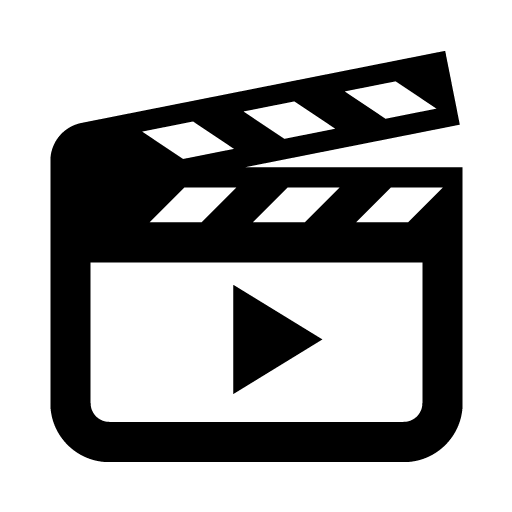
\includegraphics[width=0.15\textwidth]{05.IyA.imagenes/Video.png}}\, Campo magn\'etico terrestre

  \href{https://www.youtube.com/watch?v=UujmN0cZlSw}{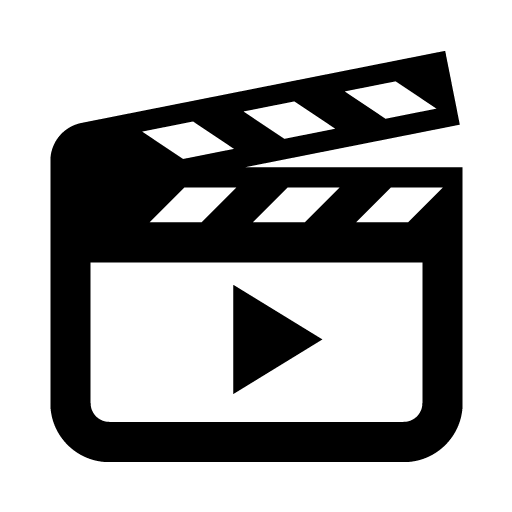
\includegraphics[width=0.15\textwidth]{05.IyA.imagenes/Video.png}}\, Sat\'elites que estudian el campo magn\'etico de la Tierra

    \href{https://www.youtube.com/watch?v=DwshhZq6T8Q}{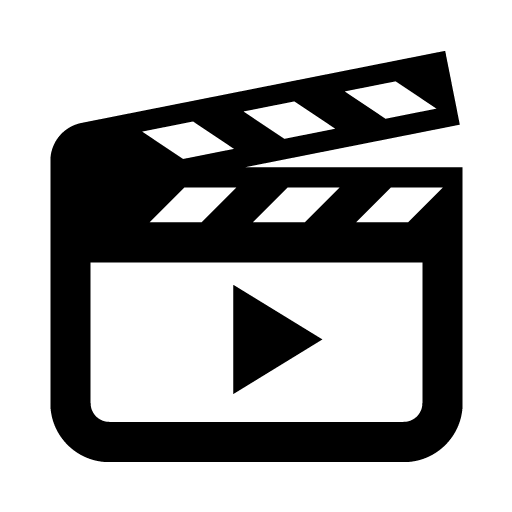
\includegraphics[width=0.15\textwidth]{05.IyA.imagenes/Video.png}}\, Magnetismo terrestre
  \end{column}
  \begin{column}{0.7\textwidth}
    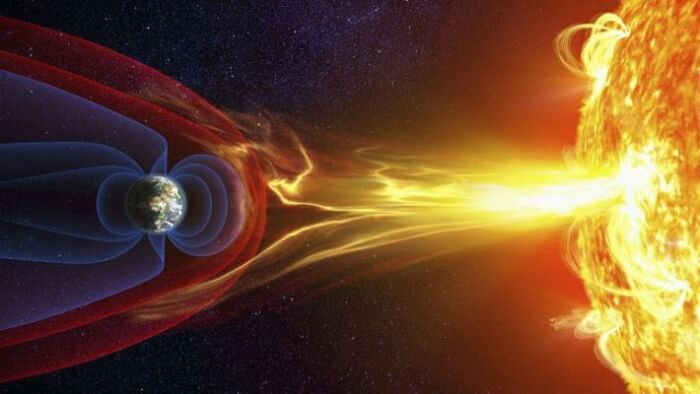
\includegraphics[width=\textwidth]{05.instrumentos.giroscopicos.imagenes/05.04.MagnetismoTerrestre/05-04-campo-magnetico-terrestre.jpg}\vspace{3mm}

    {\tiny Fuente: \url{https://www.capasdelatierra.org/campo-magnetico-magnetosfera/}}
    \end{column}
  \end{columns}
\end{frame}


\begin{frame}

  \begin{exampleblock}{Funci\'on principal del CMT }
    Proteger al planeta Tierra del viento solar
  \end{exampleblock}

  \begin{block}{Caracter\'isticas del CMT}
    \begin{itemize}{\small
    \item El proceso que lo origina se conoce como {\bf geod\'inamo} (hip\'otesis del d\'inamo)
    \item El primero en estudiarlo fue Karl Friedrich Gauss en el siglo XIX
    \item Su intensidad es m\'inima cerca del ecuador y m\'axima cerca de los polos
    \item Es una estructura din\'amica que responde a la actividad del Sol
    \item Los polos geogr\'aficos no coinciden con los magn\'eticos, se mueven en el tiempo
    \item Han existido ``{\it inversiones}'' del campo en la historia del planeta, aproximadamente
      en 20000000 de a\~nos se han invertido cada 200000 - 300000 a\~nos, la \'ultima ocurri\'o
      aproximadamente hace 780000 a\~nos
    \item La interacci\'on con el viento solar produce {\it tormentas magn\'eticas}, algunas
      part\'iculas cargadas quedan atrapadas en la magnet\'osfera y se precipitan a las regiones polares,
      chocando con mol\'eculas de ox\'igeno y nitr\'ogeno, emitiendo luz roja y verde conocidas
      como {\it auroras boreales} en latitud norte y {\it auroras australes} en latitud sur.
}
    \end{itemize}
  \end{block}\vspace{0.3mm}

{\footnotesize
Mayores detalles sobre el CMT pueden encontrarse en 
\href{https://es.gizmodo.com/como-funciona-el-campo-magnetico-de-la-tierra-en-seis-1792481678}{\TextoAzul{C\'omo funciona el campo magn\'etico de la Tierra, en seis espectaculares GIF}}
}

\end{frame}

\begin{frame}
  \begin{columns}
    \begin{column}{0.40\textwidth} \centering
      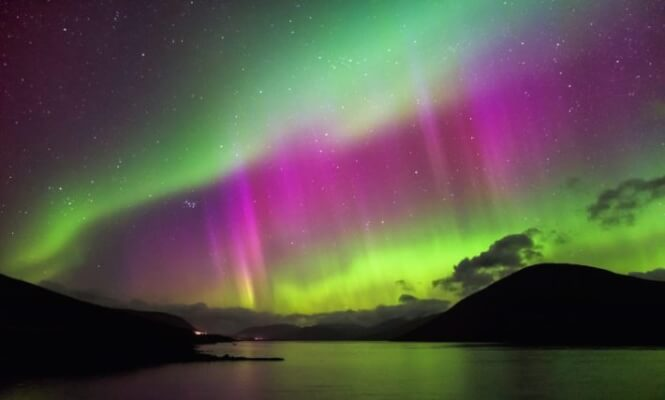
\includegraphics[width=\textwidth]{05.instrumentos.giroscopicos.imagenes/05.04.MagnetismoTerrestre/05-04-auroras.jpg}\vspace{0.3mm}
      Aurora \vspace{0.6mm}

	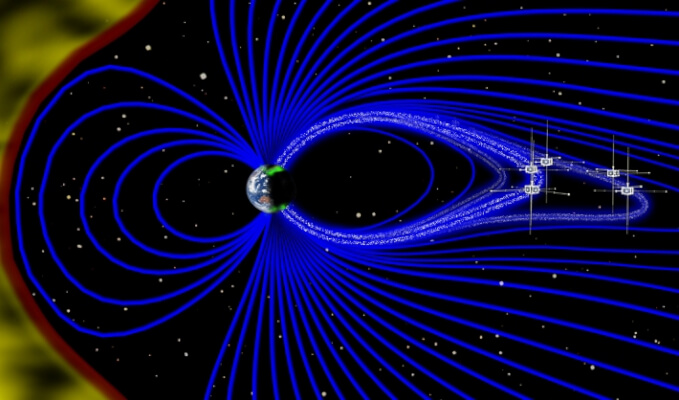
\includegraphics[width=\textwidth]{05.instrumentos.giroscopicos.imagenes/05.04.MagnetismoTerrestre/05-04-cola-del-campo-magnetico.jpeg}\vspace{0.3mm}
      Interacci\'on del CMT con el viento solar \vspace{0.6mm}

\end{column}
    \begin{column}{0.40\textwidth}

      	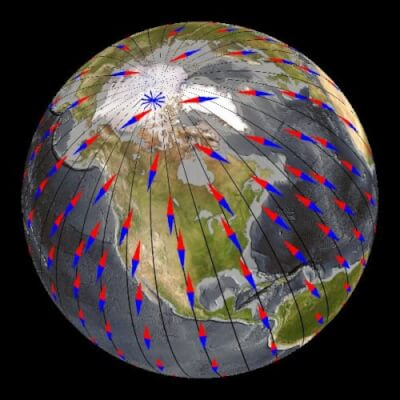
\includegraphics[width=\textwidth]{05.instrumentos.giroscopicos.imagenes/05.04.MagnetismoTerrestre/05-04-polos-de-la-tierra.jpg}
	\end{column}

\end{columns}\vspace{3mm}

    {\tiny Fuente: \url{https://www.capasdelatierra.org/campo-magnetico-magnetosfera/}}

\end{frame}

\begin{frame}
  
  \begin{columns}
    \begin{column}{0.7\textwidth}
  \begin{block}{Propiedades del CMT }{\small
    \begin{itemize}
    \item {\bf Intensidad:} resulta m\'axima en los polos y m\'inima en la zona del ecuador
	con un rango entre 25000 a 65000 nanoTesla (0,25 a 0,65 Gauss). En la actualidad se est\'a
	debilitando con una tasa de 10-15\% en los \'ultimos 150 a\~nos. Su intensidad ha subido y bajado
	en el pasado, siendo las mismas dentro de los valores obtenidos por registros de los campos magn\'eticos
	grabados en rocas.
    \item {\bf Inclinaci\'on:} se inclina hacia el suelo en la zona de los polos magn\'eticos, hasta
	quedar perpendicular a la superficie, y rota progresivamente hasta quedar horizontal al suelo 
	en el ecuador magn\'etico. En un mapa las l\'ineas de igual inclinaci\'on magn\'etica 
	se denominan {\it isoclinas}, del griego {\it isoklines = puntos de la tierra con igual inclinaci\'on
	magn\'etica}
    \item {\bf Declinaci\'on:} 
	En un mapa las l\'ineas de igual declinaci\'on magn\'etica 
	se denominan {\it isogonas}, del griego {\it isogonios = cuerpo geom\'etrico de \'angulos iguales}
    \item {\bf Dipolaridad:} el campo magn\'etico presenta un polo norte y otro sur, que no coinciden
	con los polos geogr\'aficos, y su ubicaci\'on es variable en el tiempo.
    \end{itemize}
  }
\end{block}
\end{column}
\begin{column}{0.3\textwidth}
  \begin{center}
    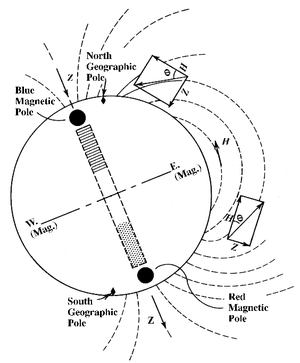
\includegraphics[width=\textwidth]{05.instrumentos.giroscopicos.imagenes/05.04.MagnetismoTerrestre/05-04-desviacion_polos.png}\\
    Inclinaci\'on del CMT
  \end{center}
\end{column}
\end{columns}

\end{frame}

\begin{frame}

  \begin{block}{Variaciones del CMT}{\small
    \begin{itemize}
    \item {\bf Variaciones temporales de corto plazo:} variaciones peri\'odicas en la fuente que genera
	al CMT o de fen\'omenos exteriores.
    \item {\bf Variaciones temporales de largo plazo:} al superar un (1) a\~no terrestre de duraci\'on,
	se las conoce como \TextoRojo{Variaciones Seculares}. Son causadas por dos tipos de procesos que tienen lugar en el n\'ucleo terrestre. El primero est\'a  relacionado con las variaciones del campo principal de un dipolo y opera con escalas de tiempo de cientos o miles de a\~nos. El segundo se relaciona con las variaciones del campo no dipolar, en escalas de tiempo del orden de decenas de anos.
    \item {\bf Inversi\'on de campo:} seg\'un se explic\'o anteriormente
    \end{itemize}
}
  \end{block}
\vspace{0.3mm}
Se puede obtener mucha informaci\'on sobre estos temas y tambi\'en planos actualizados en  \href{https://www.ngdc.noaa.gov/ngdc.html}{\TextoAzul{National Ocean and Atmospheric Administration}}

\end{frame}

\begin{frame}{Mapa Intensidad de CMT}
    
 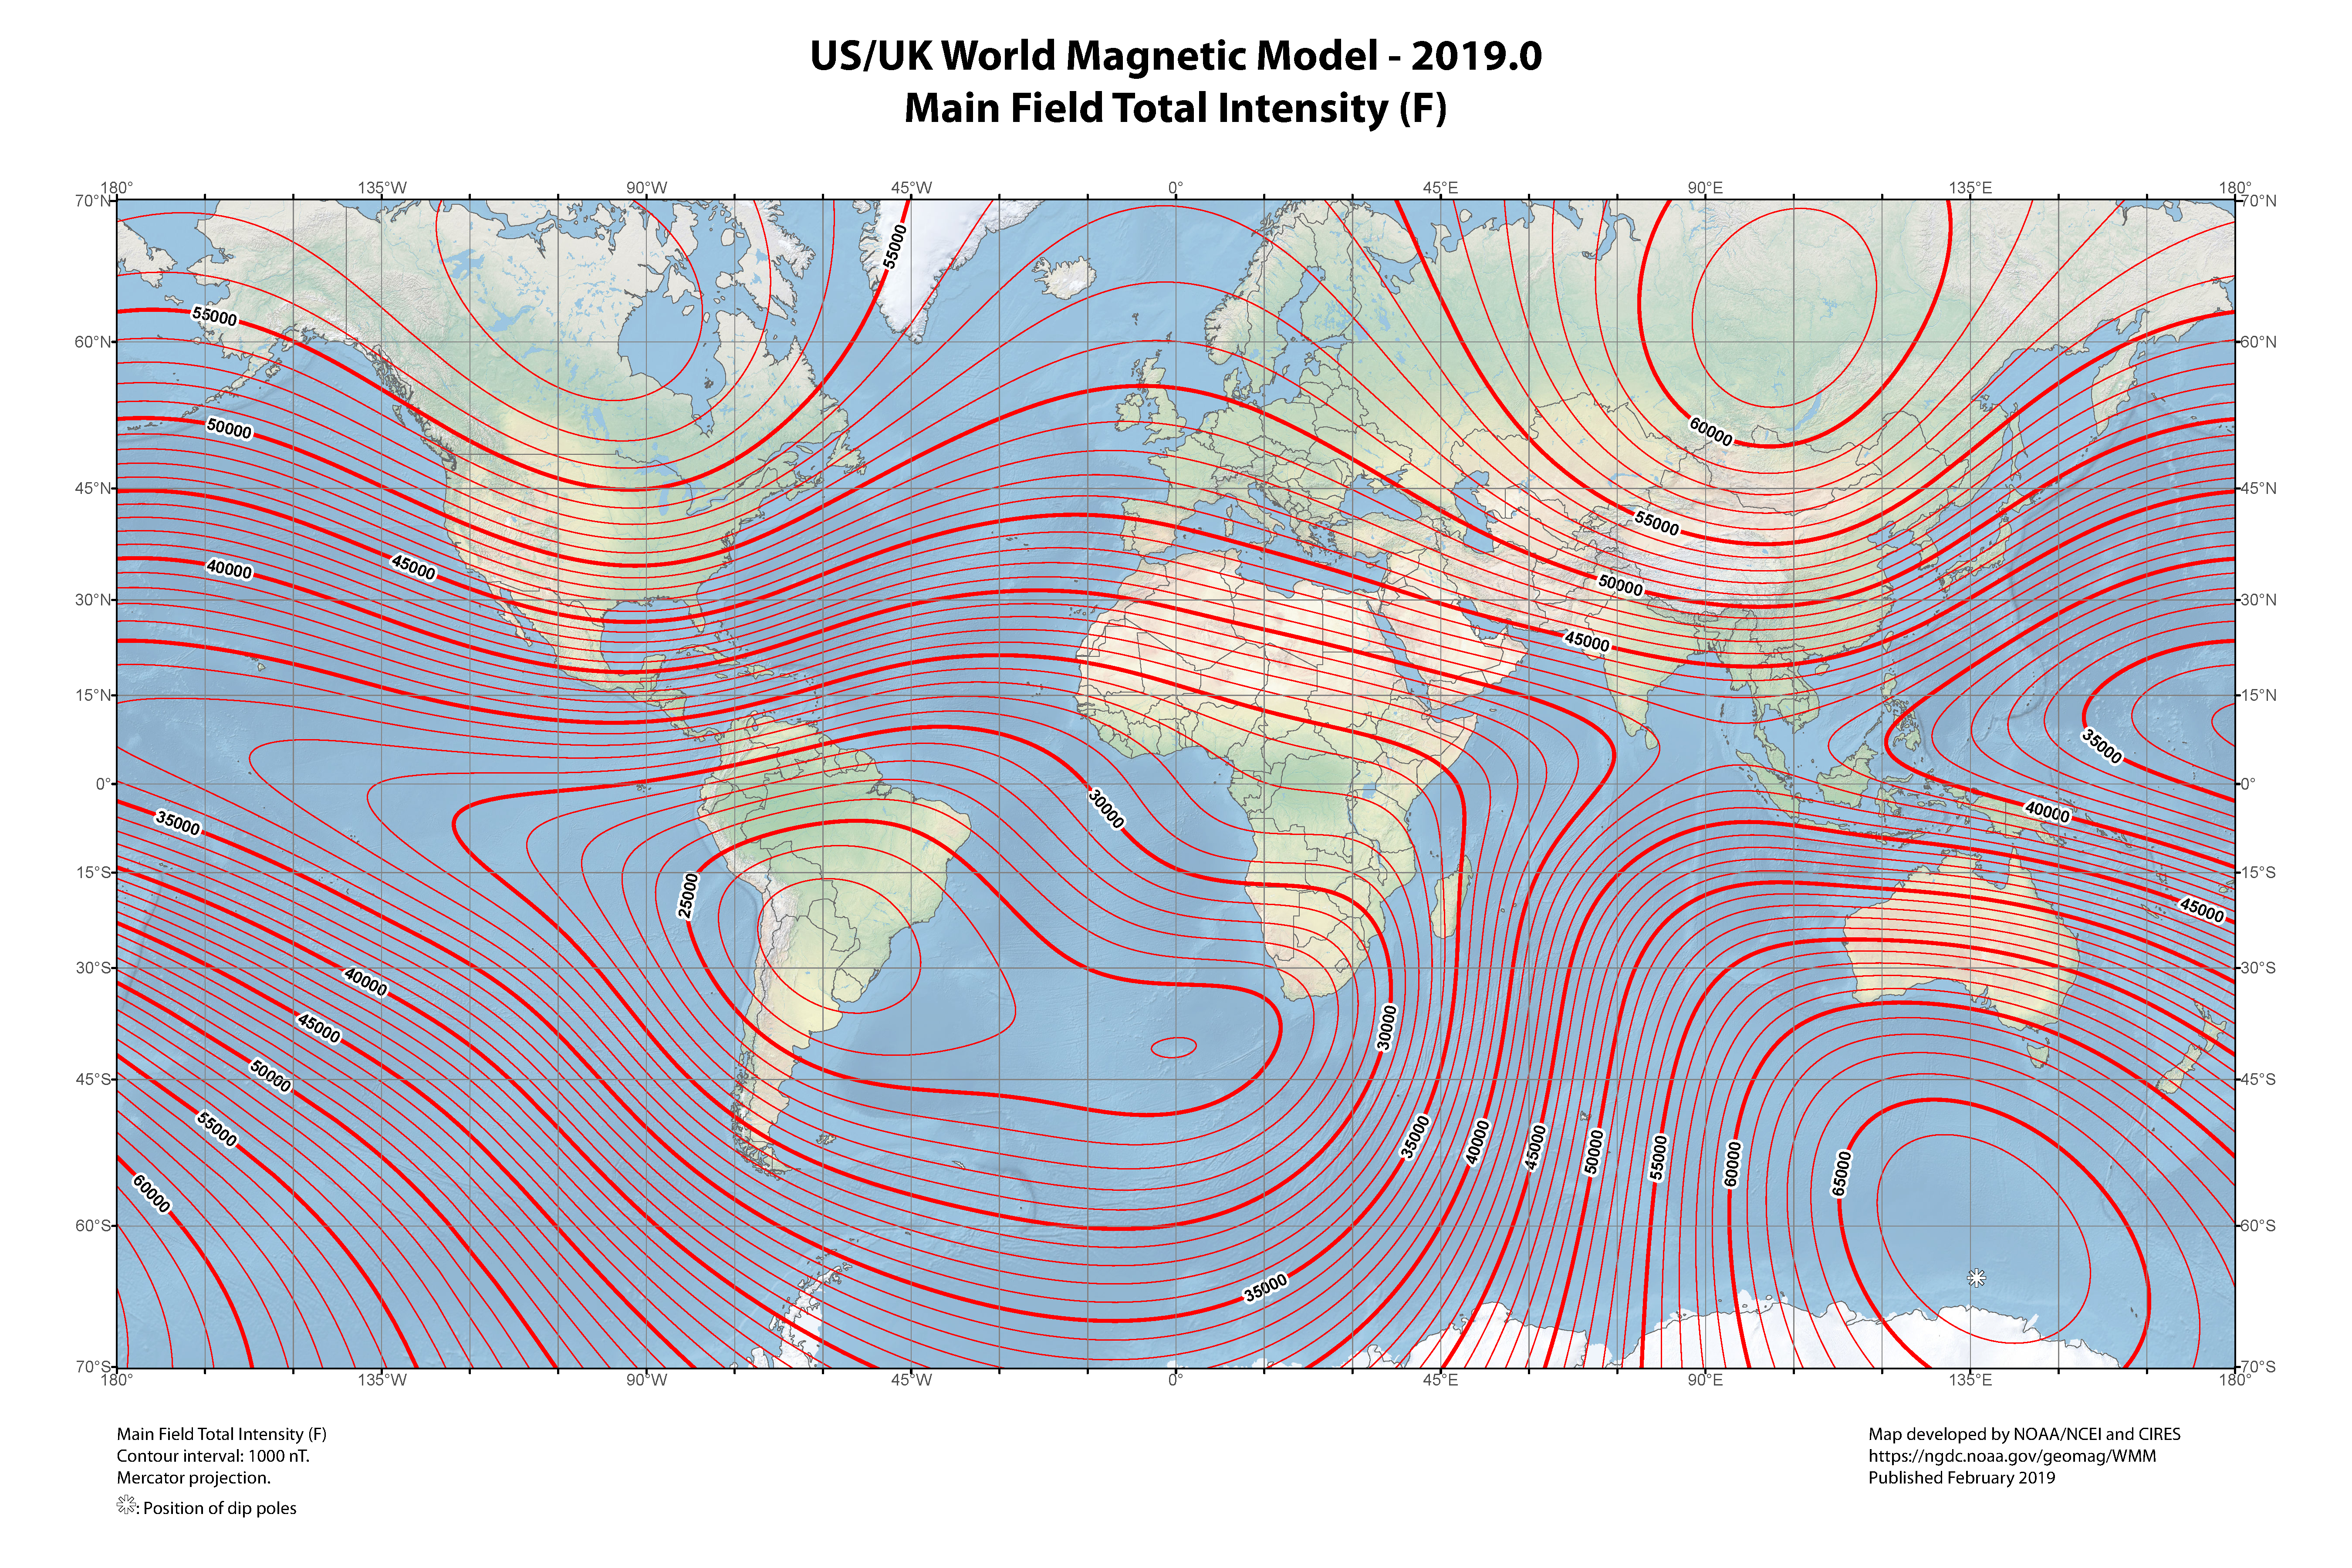
\includegraphics[width=\linewidth]{05.instrumentos.giroscopicos.imagenes/05.04.MagnetismoTerrestre/05-04-mapa_intensidad.pdf}  

\end{frame}

\begin{frame}{L\'ineas Isoclinas}
  
 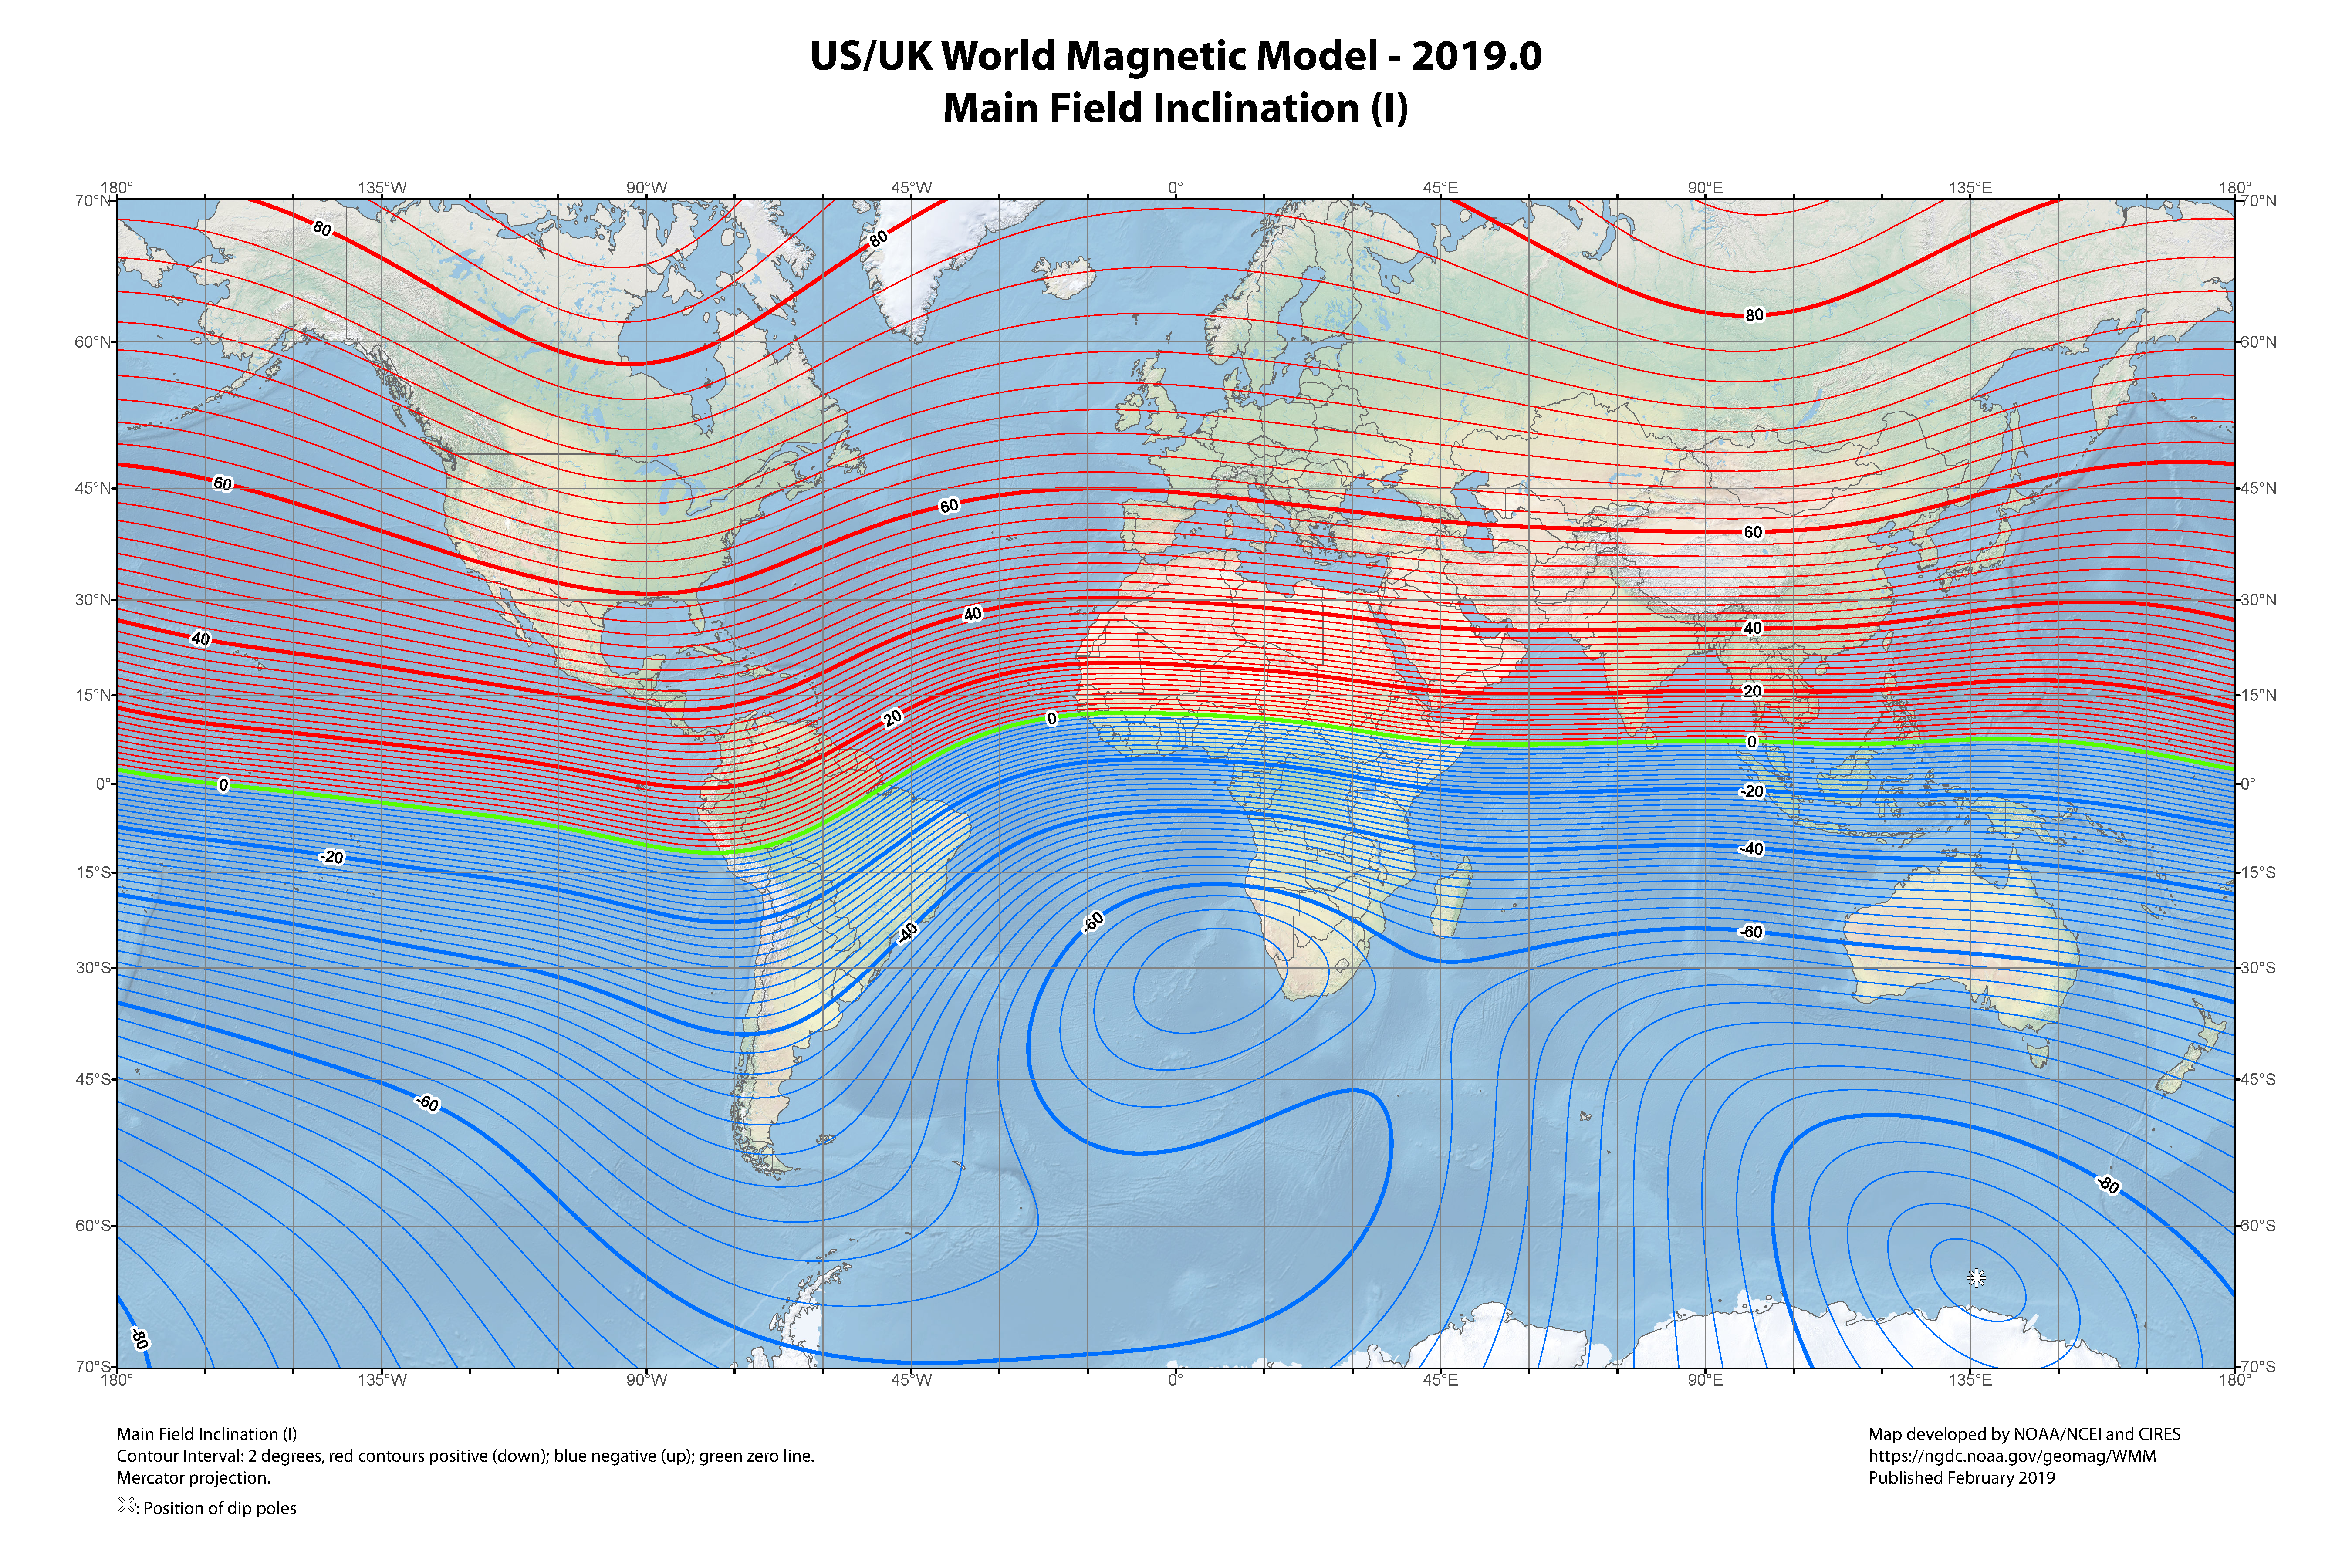
\includegraphics[width=\linewidth]{05.instrumentos.giroscopicos.imagenes/05.04.MagnetismoTerrestre/05-04-mapa_inclinacion.pdf}

\end{frame}

\begin{frame}{L\'ineas Is\'ogonas}
  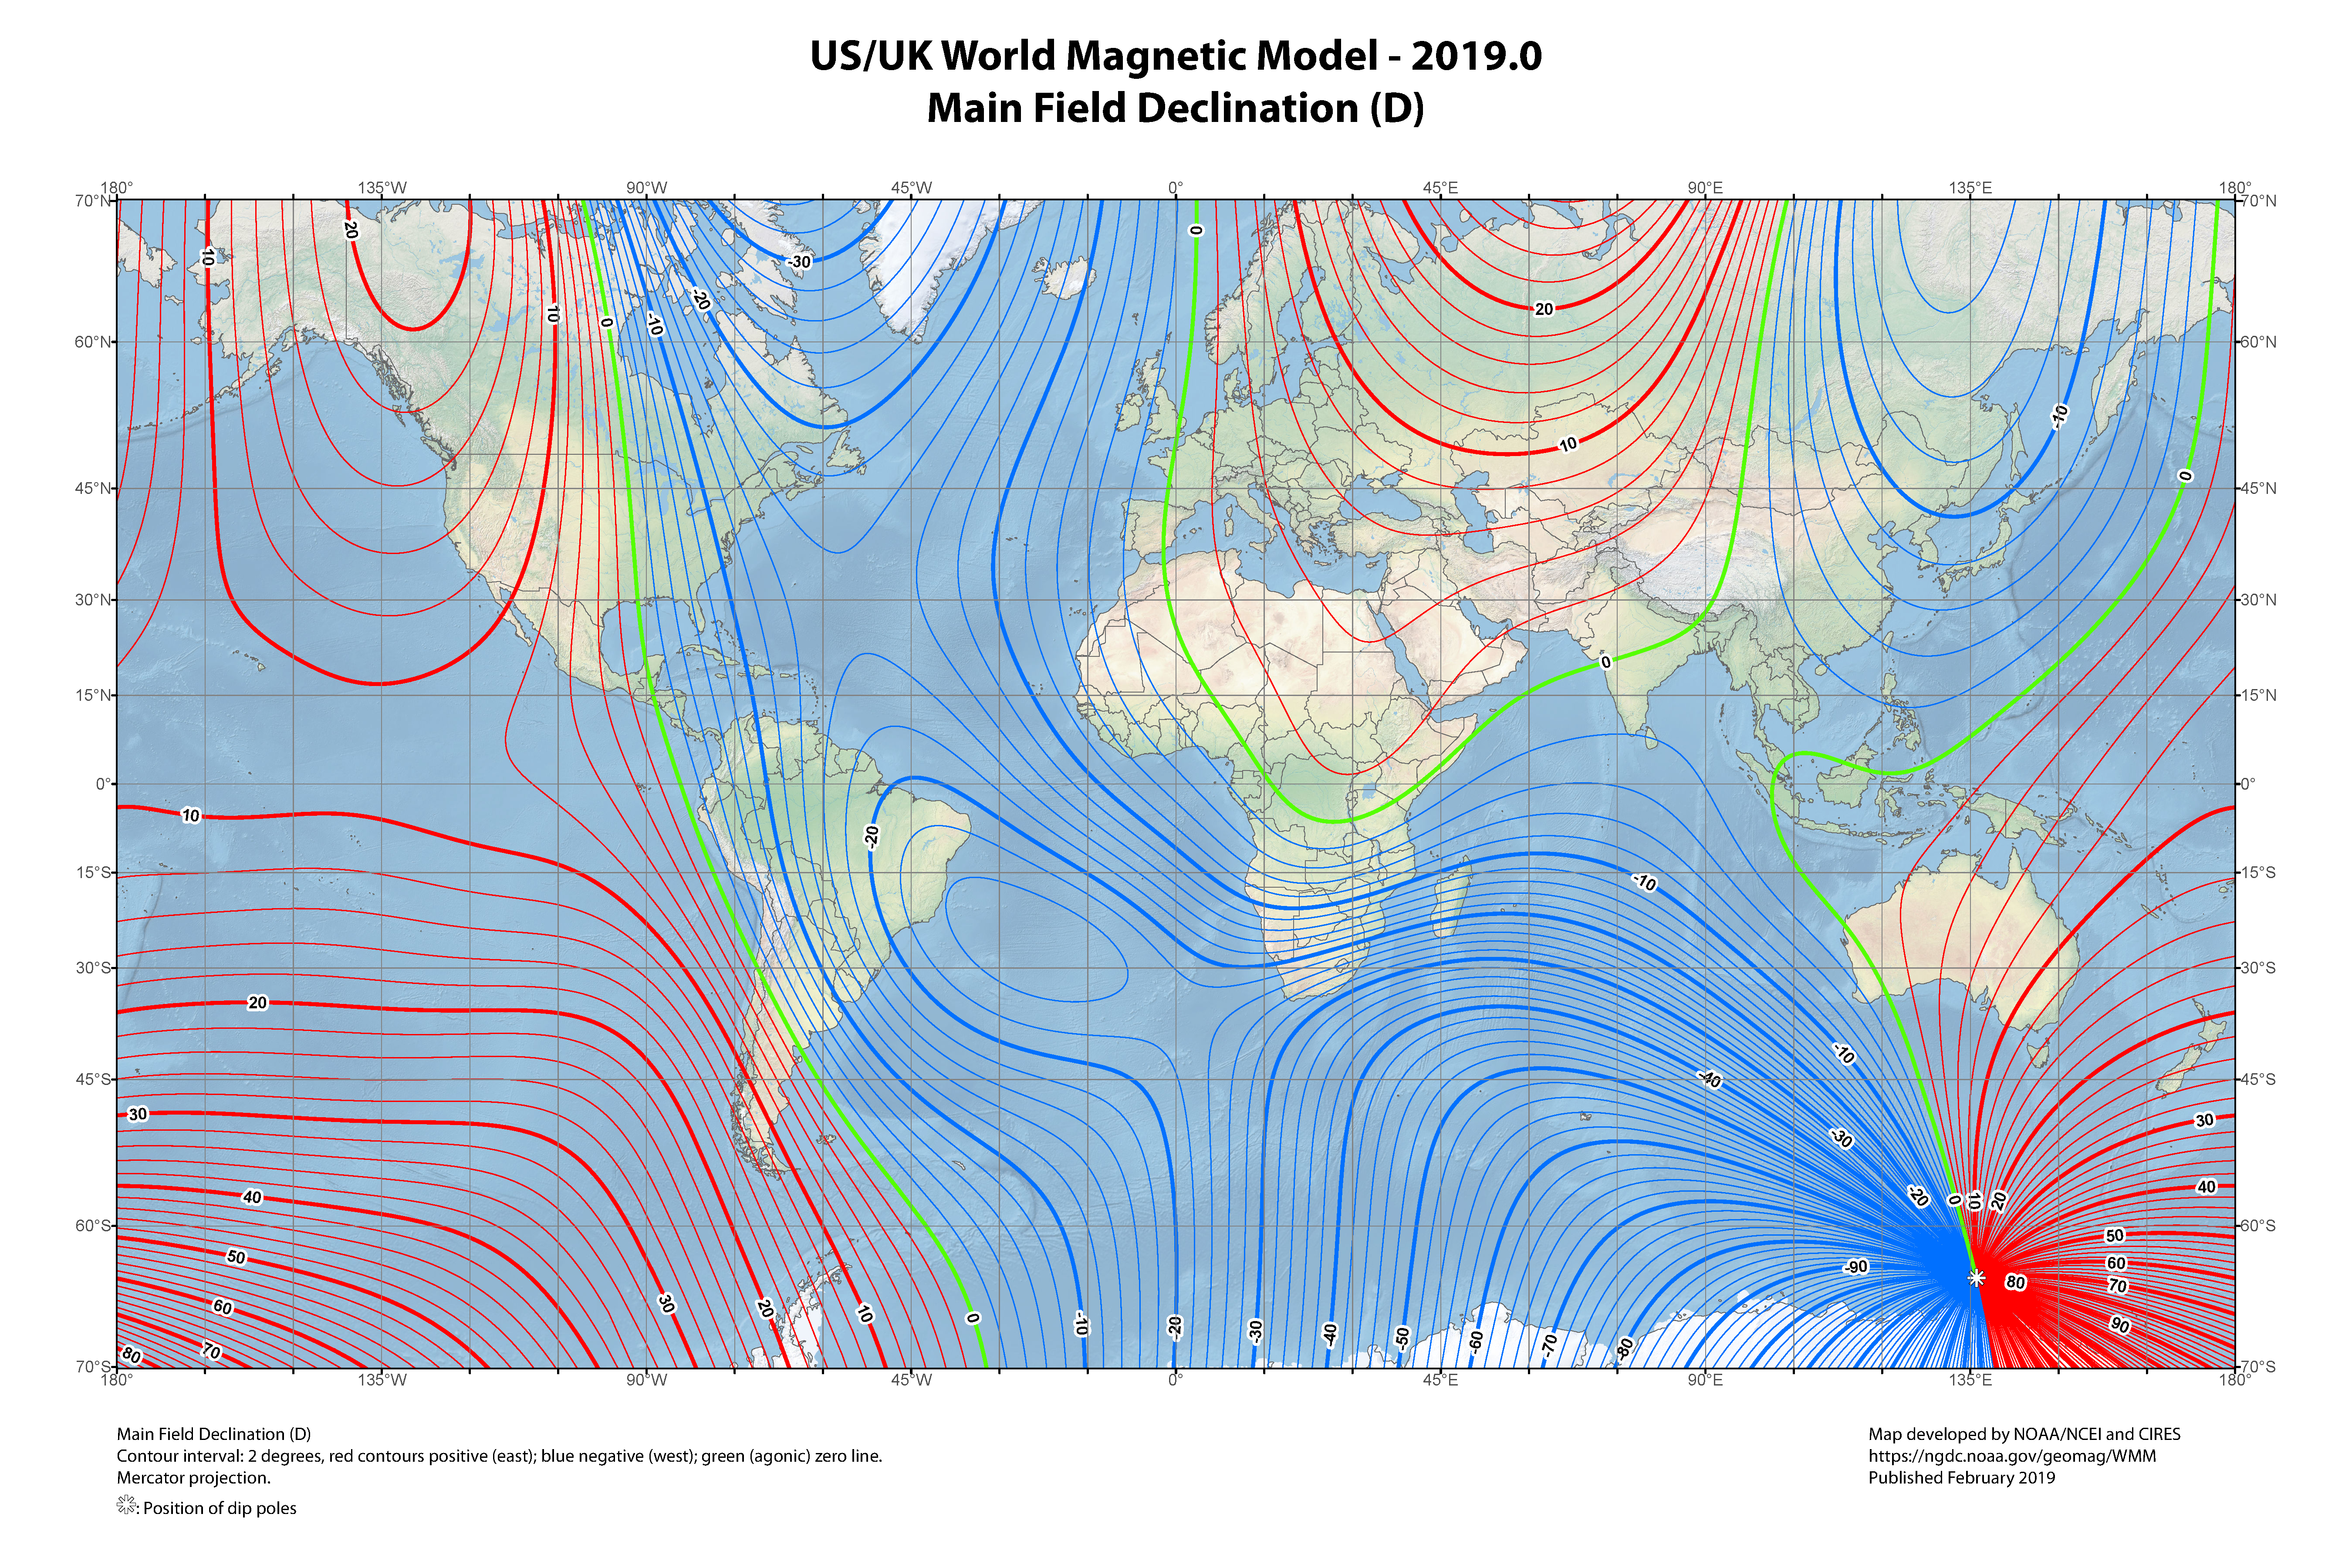
\includegraphics[width=\linewidth]{05.instrumentos.giroscopicos.imagenes/05.04.MagnetismoTerrestre/05-04-mapa_declinacion_2019.pdf}

  {\tiny Fuente: \url{https://www.ngdc.noaa.gov/ngdc.html}
  }
  
\end{frame}

% \begin{frame}{L\'ineas Is\'ogonas}
%   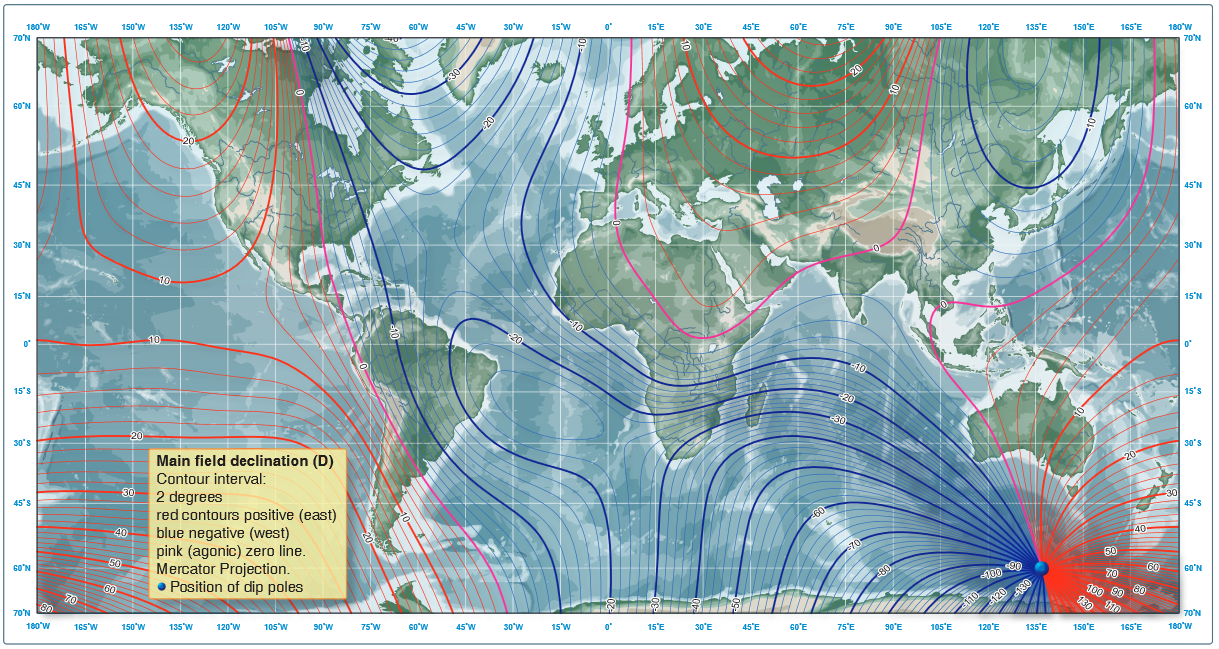
\includegraphics[width=\linewidth]{05.instrumentos.giroscopicos.imagenes/05.04.MagnetismoTerrestre/05-04-isogonic-lines-of-variation.png}

%   {\tiny Fuente: \url{https://www.cfinotebook.net/notebook/avionics-and-instruments/magnetic-compass}
%   }
  
% \end{frame}


\begin{frame}
  
  \begin{block}{Aplicaciones del CMT }
    \begin{itemize}
    \item Los animales vivos pueden detectarlo y lo utilizan para orientarse durante sus migraciones (\TextoVerde{magnetorrecepci\'on})
    \item En la navegaci\'on, mar\'itima o a\'erea, para orientarse desde el siglo XII
    \item Estudio de estructuras geol\'ogicas subterr\'aneas
    \end{itemize}
  \end{block}


\end{frame}

\begin{frame}{Forma constructiva  br\'ujula magn\'etica}

    \begin{center}
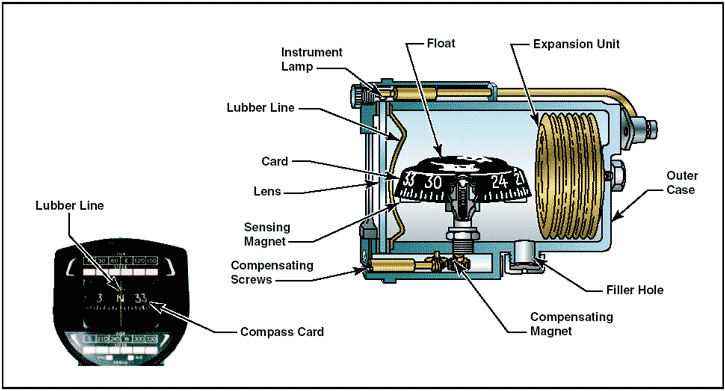
\includegraphics[width=\textwidth]{05.instrumentos.giroscopicos.imagenes/05.04.MagnetismoTerrestre/05-04-brujula_magnetica_construccion.png}
\end{center}

\end{frame}

\begin{frame}{Forma constructiva  br\'ujula magn\'etica}

    \begin{center}
      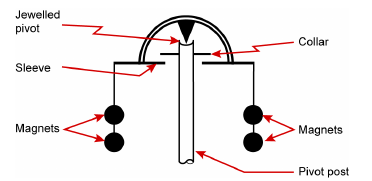
\includegraphics[width=0.56\textwidth]{05.instrumentos.giroscopicos.imagenes/05.04.MagnetismoTerrestre/05-04-brujula_magnetica.png}
      \qquad
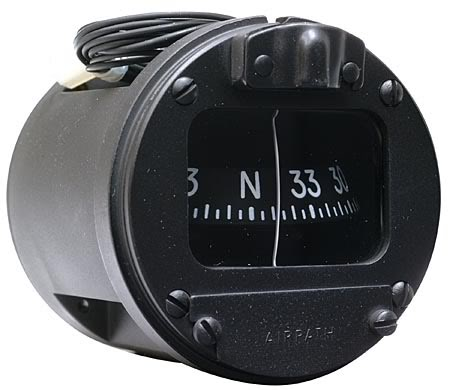
\includegraphics[width=0.35\textwidth]{05.instrumentos.giroscopicos.imagenes/05.04.MagnetismoTerrestre/05-04-MagneticCompass.jpg}      
\end{center}

\begin{block}{Propiedades}

\begin{multicols}{3}
    \begin{itemize}
         \item Horizontabilidad
         \item Sensibilidad
         \item Aperiodicidad
    \end{itemize}
\end{multicols}
\end{block}

\end{frame}

\begin{frame}{  Br\'ujula magn\'etica. Horizontabilidad }

%    \begin{center}
  \begin{columns}

    \begin{column}{0.65\textwidth}
      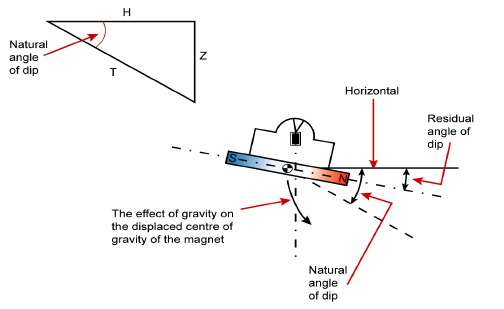
\includegraphics[width=\linewidth]{05.instrumentos.giroscopicos.imagenes/05.04.MagnetismoTerrestre/05-04-brujula_magnetica_inclinacione.png}
    \end{column}
    
    \begin{column}{0.4\textwidth}

    \begin{alertblock}{Requerimiento}
      Resulta escencial que la br\'ujula se mantenga lo m\'as cercano posible al plano horizontal
    \end{alertblock}

    \begin{exampleblock}{Soluci\'on}
      Mediante la forma constructiva y de suspensi\'on en forma de p\'endulo, con su centro de gravedad
      por debajo del punto de suspensi\'on.\\
      El \'angulo residual de inclinaci\'on puede ser $< 3$º
    \end{exampleblock}

    \end{column}
    
  \end{columns}


%    \end{center}

    % It is therefore essential that the compass magnets should lie as close as possible to the horizontal plane

\end{frame}

\begin{frame}{  Br\'ujula magn\'etica. Sensibilidad }

%   Sensitivity is a measure of the ability of the compass magnetic assembly to point accurately
%   towards north.
%   Nothing can be done to increase the strength of the weak terrestrial magnetic field and so it is
% necessary to use several magnets with high pole strengths. The magnetic assembly is made as light as
% possible to reduce friction at the pivot.
% 9.
% The pivot itself normally incorporates a jewelled bearing which is lubricated by the viscous
% fluid which fills the bowl. Being fairly dense the fluid effectively lightens the magnet assembly still
% further, once again reducing friction at the pivot.

  La sensibilidad es una medida de la habilidad del instrumento para indicar con precisi\'on hacia el norte.

  Dado que no puede aumentarse la intensidad del CMT, se utilizan varios imanes de gran intensidad y
  se reduce todo lo posible la fricci\'on en el punto de pivote.
  Este usualmente es una piedra preciosa lubricado por el l\'iquido que contiene el instrumento que, al
  ser cierta densidad, permite una cierta flotaci\'on de la carta, reduciendo la fricci\'on.
  
  \begin{center}
  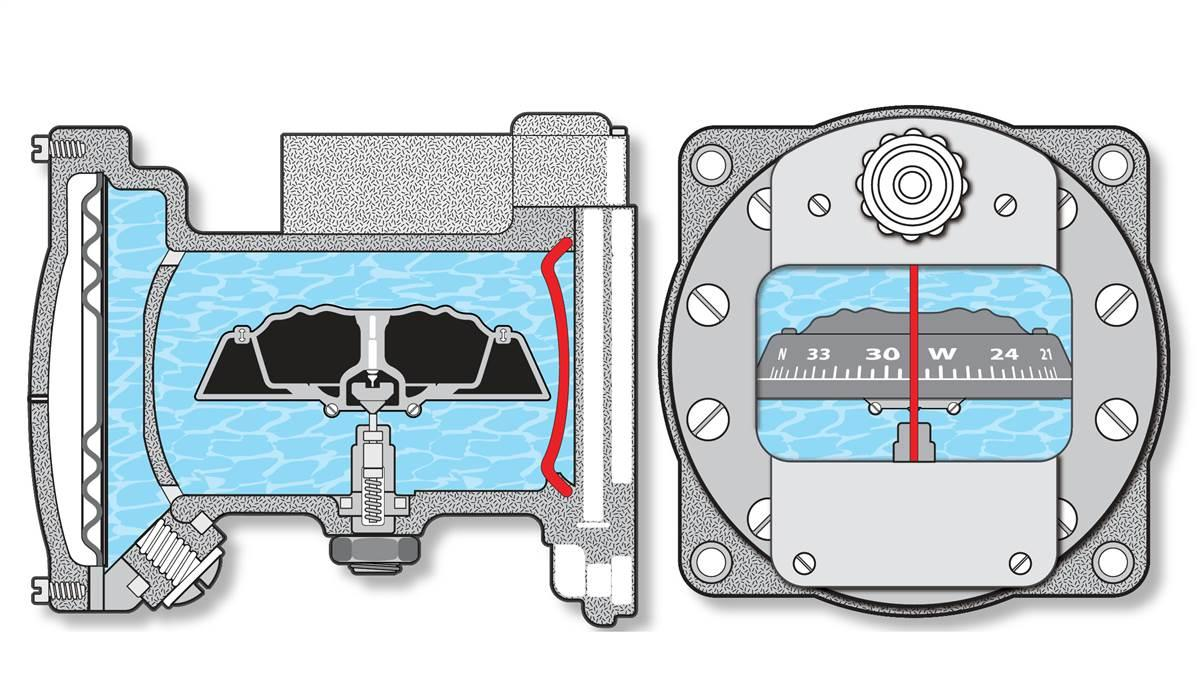
\includegraphics[width=0.7\textwidth]{05.instrumentos.giroscopicos.imagenes/05.04.MagnetismoTerrestre/05-04-1704f_pf_hiw_16x9.jpg}
\end{center}

  
\end{frame}

 \begin{frame}{  Br\'ujula magn\'etica. Aperiodicidad }

 La aperiodicidad se define como la habilidad del sistema para amortiguar r\'apidamente las oscilaciones, apuntando hacia el polo norte magn\'etico, despu\'es de un desplazamiento por maniobras o turbulencias.
  
 Si una br\'ujula magn\'etica no es enteramente aperi\'odica, el efecto es que su indicaci\'on oscila alrededor del norte magn\'etico, llegando a descansar s\'olo lentamente.

 La aperiodicidad se logra utilizando imanes peque\~nos, manteniendo la masa del conjunto oscilante
 cerca de su punto pivote y reduciendo el momento de inercia total. Esto puede lograrse utilizando
 materiales ligeros en la parte m\'ovil y mediante la viscosidad del fluido amortiguante. \'Este
 fluido debe ser transparente y  llenar completamente el interior del instrumento para evitar oscilaciones.
 Para \'esto se provee unas c\'apsulas de expansi\'on debido a efectos de temperatura.

 \end{frame}  

\begin{frame}{Br\'ujula magn\'etica. Distancias de seguridad}

  Uno de los mayores problemas con el comp\'as magn\'etico es que resulta de lectura directa, por lo
  que debe ubicarse en la cabina del piloto y, por lo tanto, se encuentra rodeado por
  equipos que pueden causarle desviaci\'on a su indicaci\'on.

  Por lo anterior, debe estudiarse cuidadosamente la ubicaci\'on del instrumento.

  Como recomendaciones sobre la ubicaci\'on del mismo:

  \begin{itemize}
  \item Cada equipo el\'ectrico o electr\'onico cercano no debe causar una desviaci\'on
    de no mas de 1\grad en el comp\'as. La suma total de los errores de todos los equipos de este
    tipo debe ser menor a 2\grad.
  \item De la misma manera, los cables de conexi\'on de cada equipo, desviaciones $< 1$\grad, para
    todos los cables, $<2$\grad.
  \item La operaci\'on de los equipos en cabina, desviaci\'on $< 1$\grad
  \item Cuando el comp\'as magn\'etico es el instrumento principal para el rumbo, la desviaci\'on
    m\'axima de cualquier rumbo $< 3$\grad.
  \end{itemize}
 
 
 \end{frame}

\begin{frame}{Comp\'as magn\'etico de carta vertical}
  Tambi\'en conocido como tipo E.

  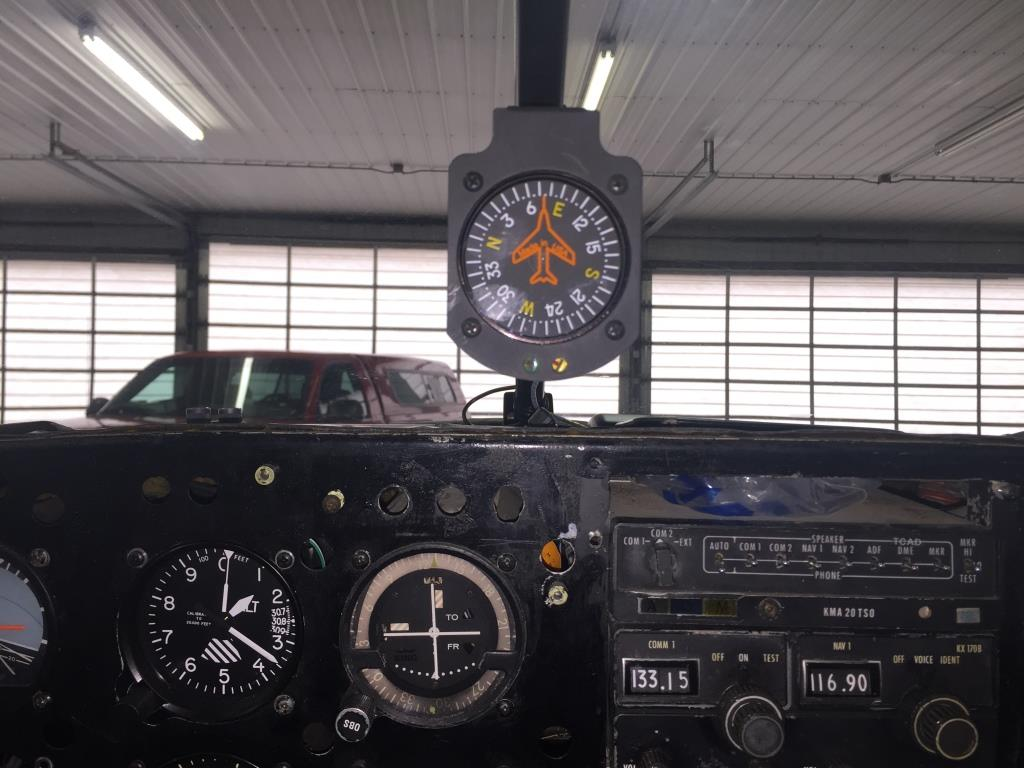
\includegraphics[width=0.35\textwidth]{05.instrumentos.giroscopicos.imagenes/05.04.MagnetismoTerrestre/05-04-IMG_6513.JPG} \hspace{1mm}
      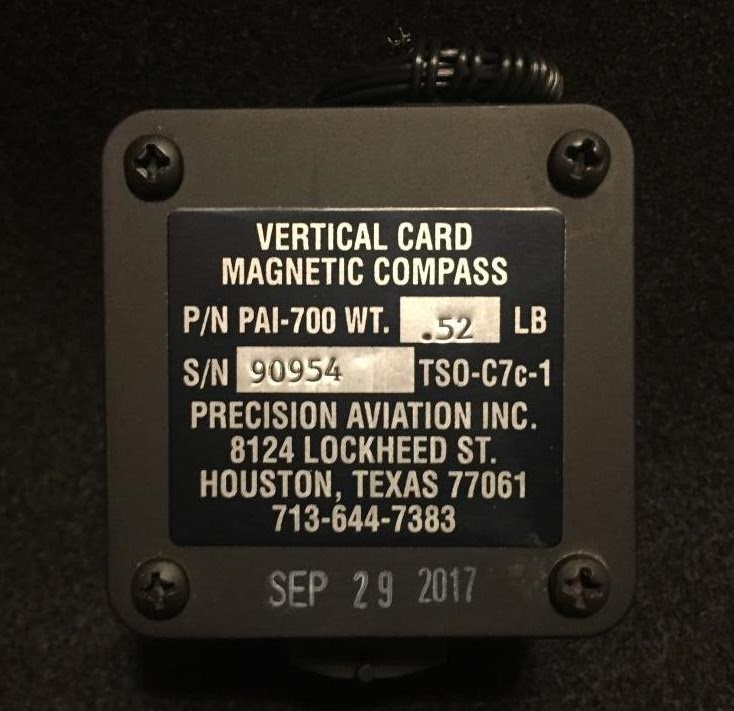
\includegraphics[width=0.25\textwidth]{05.instrumentos.giroscopicos.imagenes/05.04.MagnetismoTerrestre/05-04-IMG_6464.JPG} \hspace{1mm}
      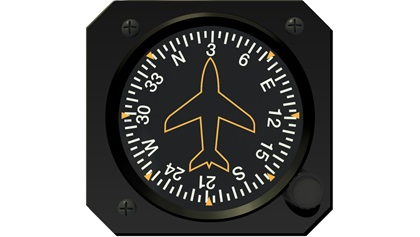
\includegraphics[width=0.45\textwidth]{05.instrumentos.giroscopicos.imagenes/05.04.MagnetismoTerrestre/05-04-VerticalCardCompass.jpg}
      
  {\tiny Fuente: \url{http://n98297.blogspot.com/2017/12/pai-700-compass-installation.html}}
\end{frame}


\begin{frame}

  \begin{alertblock}{Errores  br\'ujula magn\'etica}
    \begin{itemize}
    \item Aceleraci\'on
    \item Giro
    \item Movimiento del l\'iquido
    \end{itemize}
  \end{alertblock}

\end{frame}

\begin{frame}{Errores br\'ujula magn\'etica. Aceleraci\'on}

Debido a la inercia. 

  \begin{center}
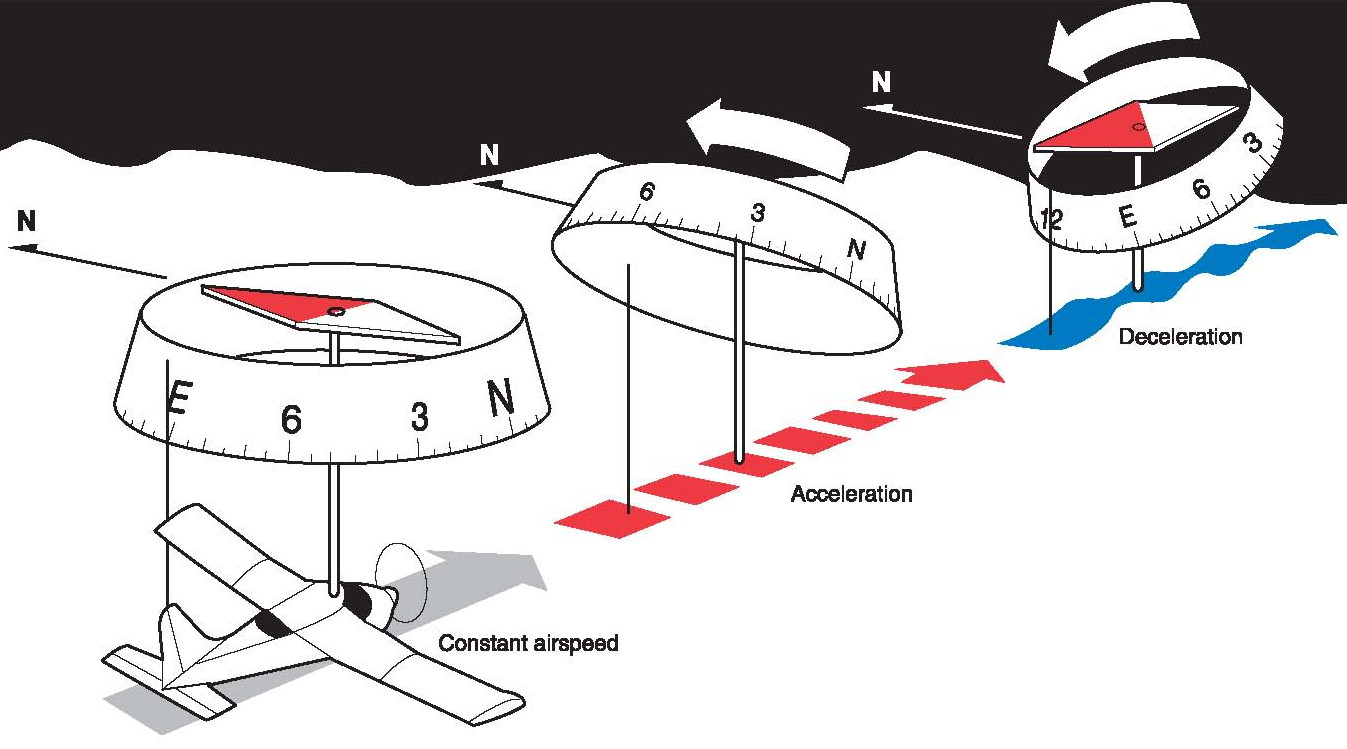
\includegraphics[width=0.80\textwidth]{05.instrumentos.giroscopicos.imagenes/05.04.MagnetismoTerrestre/05-04-brujula_error_aceleracion.jpg}
\end{center}
  
\href{https://www.youtube.com/watch?v=vUz09IpYCuY}{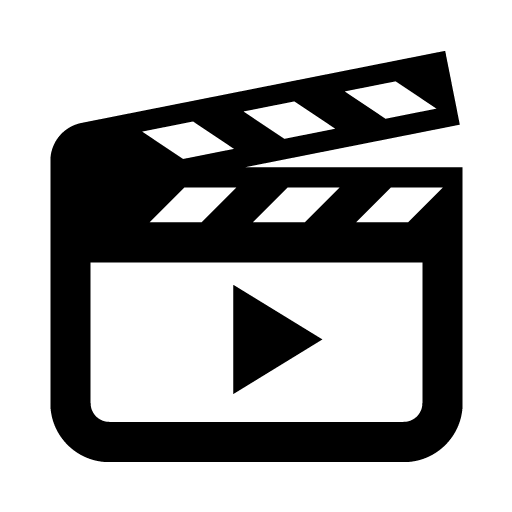
\includegraphics[width=0.10\textwidth]{05.IyA.imagenes/Video.png}}


\end{frame}

\begin{frame}{Errores br\'ujula magn\'etica. Giro}


  \begin{center}
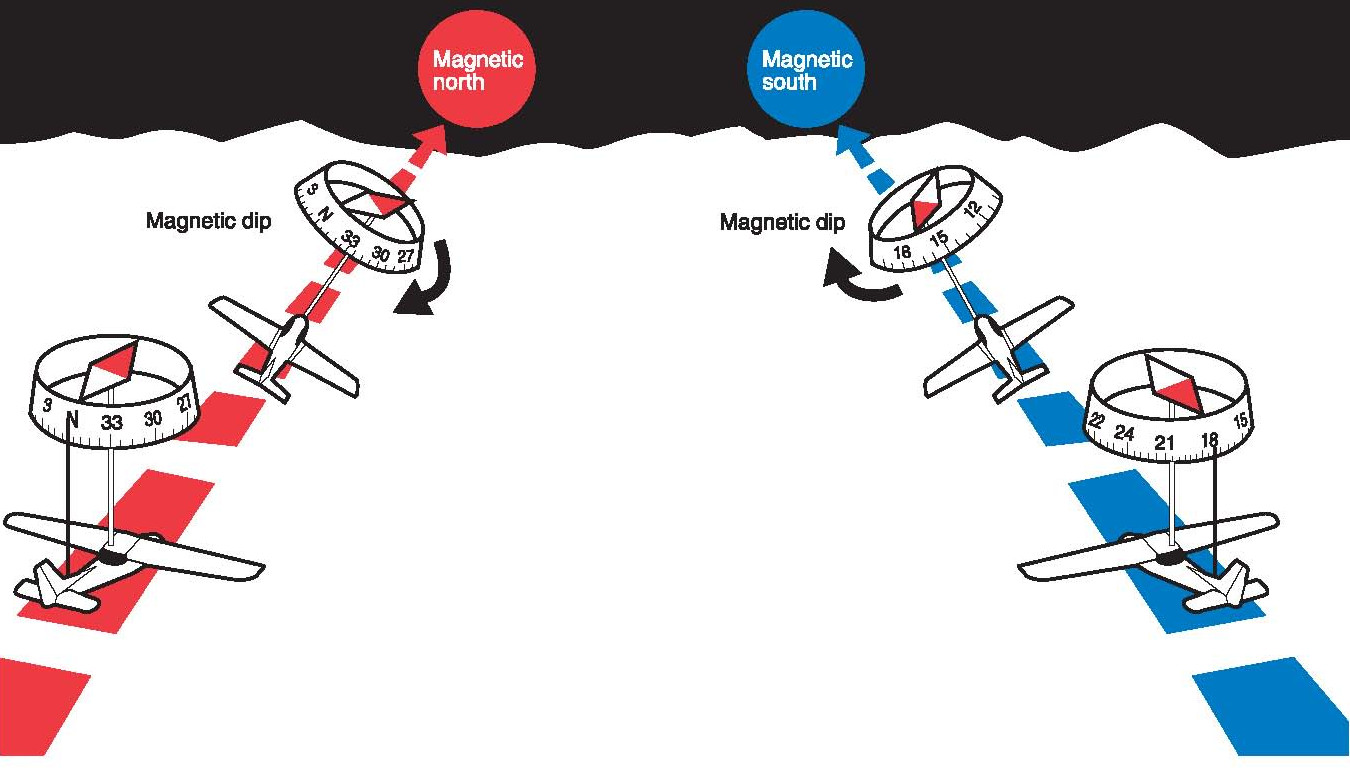
\includegraphics[width=0.80\textwidth]{05.instrumentos.giroscopicos.imagenes/05.04.MagnetismoTerrestre/05-04-brujula_error_giro.jpg}
\end{center}
  
  
\href{https://www.youtube.com/watch?v=WqXujnDw-kE}{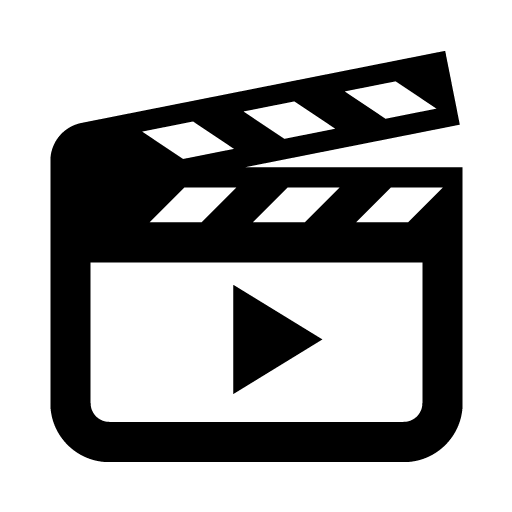
\includegraphics[width=0.10\textwidth]{05.IyA.imagenes/Video.png}}

\end{frame}